\documentclass[12pt, twoside]{article}
\usepackage[letterpaper, margin=1in, headsep=0.5in]{geometry}
\usepackage[english]{babel}
\usepackage[utf8]{inputenc}
\usepackage{amsmath}
\usepackage{amsfonts}
\usepackage{amssymb}
\usepackage{tikz}
\usetikzlibrary{quotes, angles}
\usepackage{graphicx}
\usepackage{enumitem}
\usepackage{multicol}
\usepackage{hyperref}

\newif\ifmeta
\metatrue %print standards and topics tags

\title{IB Mathematics}
\author{Chris Huson}
\date{January 2022}

\usepackage{fancyhdr}
\pagestyle{fancy}
\fancyhf{}
\renewcommand{\headrulewidth}{0pt} % disable the underline of the header
\raggedbottom


\fancyhead[LE]{\thepage}
\fancyhead[RO]{\thepage \\ Name: \hspace{4cm} \,\\}
\fancyhead[LO]{BECA / IB Math 03-Quadratic functions\\* 11 January 2022}

\begin{document}

\subsubsection*{3.7 Pre-Quiz: Linear and quadratic functions}
\begin{enumerate}
\item A linear function $f$ is graphed below. \hfill [4]
    \begin{multicols}{2}
    \begin{enumerate}
      \item Write down it's slope.\\ $m=$
      \vspace{0.25cm}
      \item Write down it's $y$-intercept.\\ $b=$
      \vspace{0.25cm}
      \item Write down the equation of the line.
      \vspace{1cm}
      \item State the coordinates of the point $Q$.
    \end{enumerate} \vspace{.5cm}
      \begin{center} 
      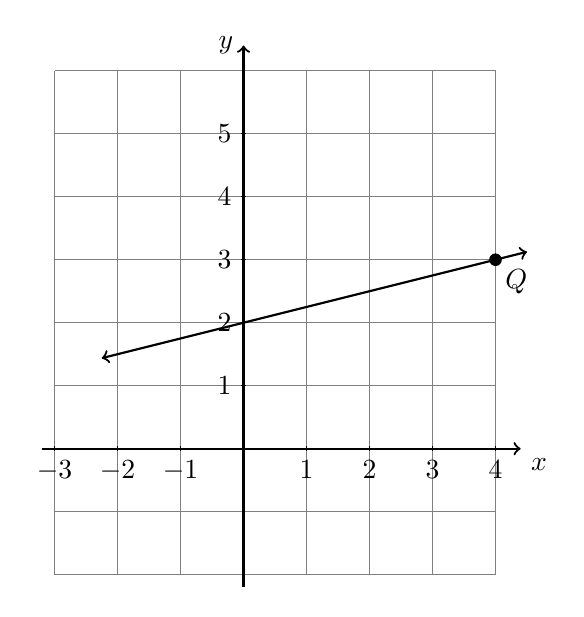
\begin{tikzpicture}[scale=0.8]
        \draw [help lines] (-3,-2) grid (4,6);
        \draw [thick, ->] (-3.2,0) -- (4.4,0) node [below right] {$x$};
        \draw [thick, ->] (0,-2.2)--(0,6.4) node [left] {$y$};
        \foreach \x in {-3,-2,-1,1,2,...,4} \draw (\x cm,1pt) -- (\x cm,-1pt) node[anchor=north] {$\x$};
        \foreach \y in {1, 2, 3, 4, 5} \draw (1pt,\y cm) -- (-1pt,\y cm) node[anchor=east] {$\y$};
        \draw [thick, <->,smooth,samples=20,domain=-2.25:4.5] plot(\x,0.25*\x+2);
        \fill (4,3) circle[radius=0.1] node[below right]{$Q$};
      \end{tikzpicture}
      \end{center}
    \end{multicols}
    
\item Write the linear equation $y-5=3(x+1)$ in the form $y=mx+c$.  \hfill [2]\vspace{4cm}

\item Given $f(x)=(x-3)(x+4)$
    \begin{enumerate}[itemsep=0.9cm]
        \begin{multicols}{2}
        \item Sketch the function. Label the vertex as an ordered pair and mark the intercepts with their values.
        \item Expand the function to standard form, $f(x)=ax^2+bx+c \text{ where } a, b, c \;  \epsilon \; \mathbb{R}$. \vspace{3.5cm}
        \begin{center}
            \begin{tikzpicture}
                \draw [thick, ->] (-3.5,0) -- (+3.5,0) node [below left] {$x$};
                \draw [thick, ->] (0,-4.5) -- (0,3) node [left] {$y$};
            \end{tikzpicture}
            \end{center}
        \end{multicols}
    \end{enumerate}

\item The function $f(x)=-x^{2}+6x-5$ is shown on the graph.
    \begin{enumerate}[itemsep=1.2cm]
      \begin{multicols}{2}
          \item Write down its vertex as an ordered pair.
          \item Write down $f(0)$.
          \item Write down two solutions to $f(x)=0$. 
          \item Hence or otherwise, write $f$ in the form $f(x)=a(x-p)(x-q)$\vspace{3cm}
          \begin{center}
          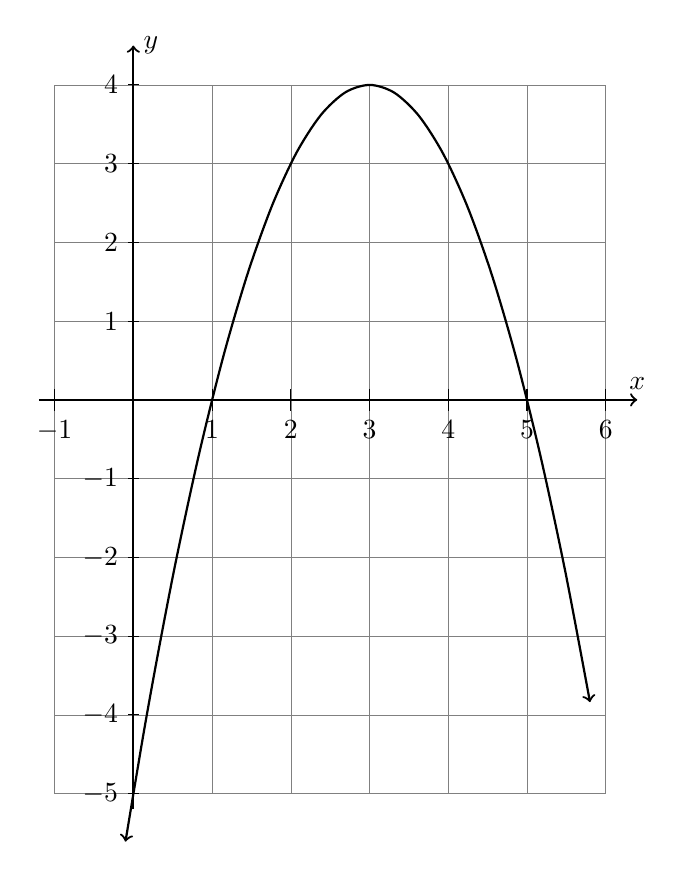
\begin{tikzpicture}[scale=1]
            \draw [help lines] (-1,-5) grid (6,4);
            \draw [thick, ->] (-1.2,0) -- (6.4,0) node [above] {$x$};
            \draw [thick, ->] (0,-5.2)--(0,4.5) node [right] {$y$};
            \foreach \x in {-1, 1,2, ...,6} \draw (\x cm,4pt) -- (\x cm,-4pt) node[below] {$\x$};
            \foreach \y in {-5,...,-1,1,2,...,4} \draw (2pt,\y cm) -- (-2pt,\y cm) node[left] {$\y$};
            %\fill (-1,0) circle[radius=0.1] node[above left]{$j$};
            %\fill (3,0) circle[radius=0.1] node[above right]{$k$};
            \draw [thick, <->,smooth,samples=20,domain=-0.1:5.8] plot(\x,-\x*\x+6*\x-5);
          \end{tikzpicture}
          \end{center}
        \end{multicols}
    \end{enumerate} \vspace{2cm}
    
\item Consider the function $f(x)=x^2+2x-3$.
\begin{enumerate}
    \item Sketch the graph of $f$, for $-4 \leq x \leq 2$. Label the vertex and the intercepts.
    \item This function can also be written in the form $f(x)=(x-p)^2 -4$.\\* 
    Write down the value of $p$. \vspace{1.5cm}
    \item The graph of $f$ has two solutions for $f(x)=0$. Write down the solutions (or roots, zeros) of the function. \vspace{1.5cm}
    \item Hence, write down the function in factored form, $f(x)=(x-a)(x-b)$. \vspace{1.5cm}
\end{enumerate}
    
\newpage
\item Given two functions, a quadratic function $f(x)=0.6x^2-2.4x-8$ and a linear function $g(x)=0.6x-4.4$.
    \begin{enumerate}%[itemsep=1cm]
        \item Graph the parabola $y=f(x)$, marking the $y$-intercept and the vertex as an ordered pair.
        \item Find the coordinates of the two intercepts with the $x$-axis, the roots or zeros of $f(x)$.\vspace{1cm}
        \item Plot the linear function, $y=g(x)$. Mark and label the two intersections of the two functions $f(x)=g(x)$ as ordered pairs.
    \end{enumerate}
    \begin{center}
    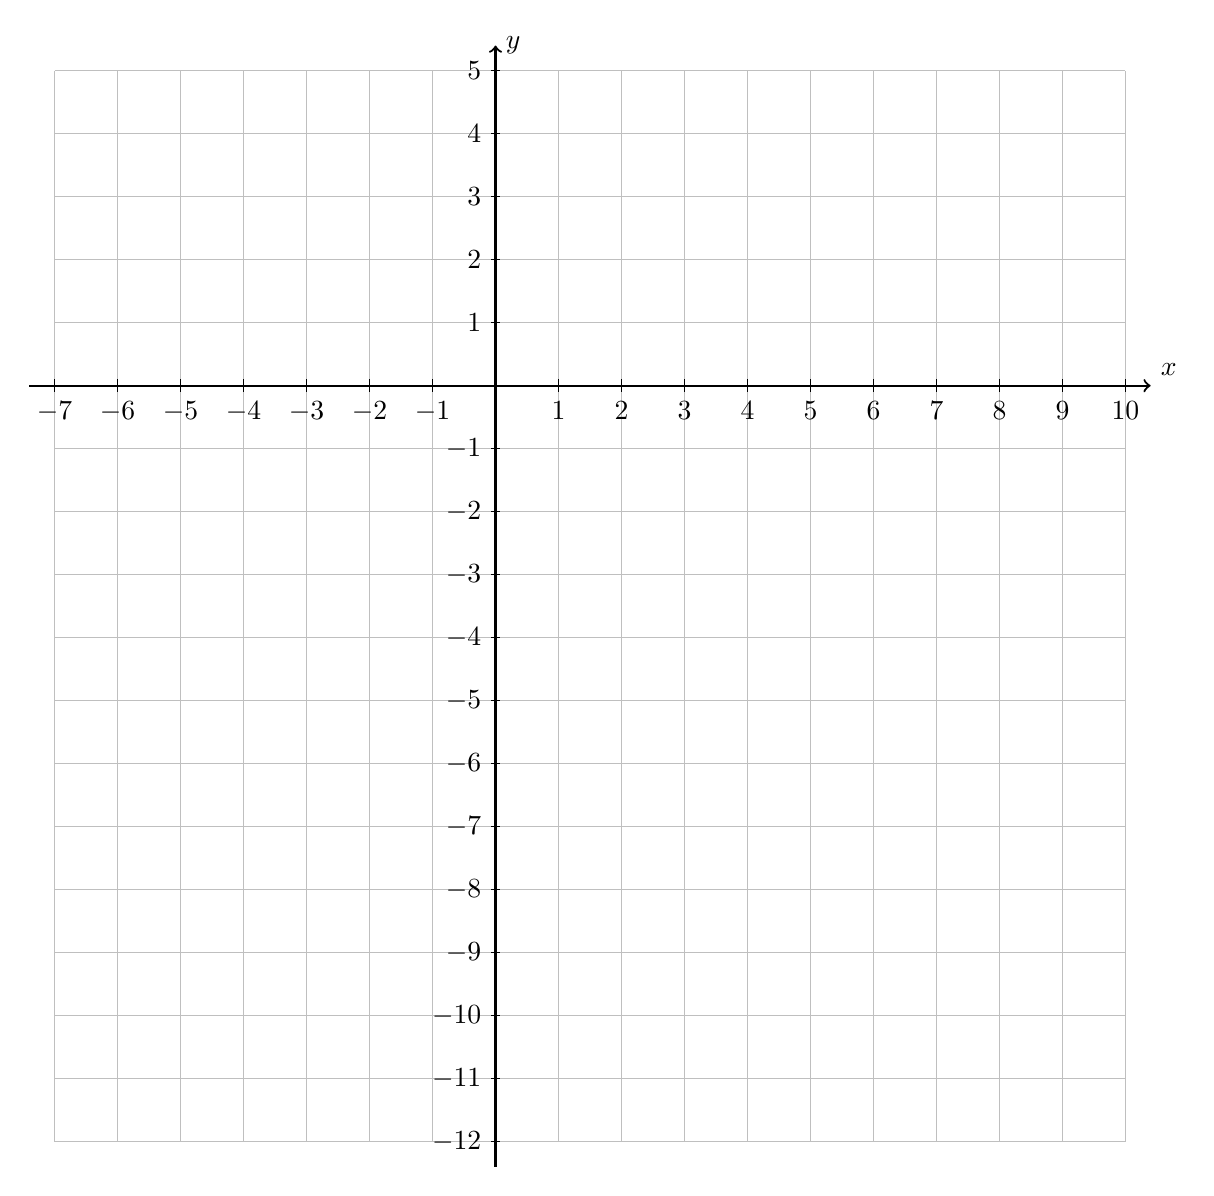
\begin{tikzpicture}[scale=0.8]
        \draw [thin, color=lightgray,, xstep=1.0cm,ystep=1.0cm] (-7,-12) grid (10,5);
        \foreach \x in {-7,...,-1,1,2,...,10}
        \draw (\x cm,3pt) -- (\x cm,-3pt) node[below] {$\x$};
        \foreach \y in {-12,...,-1,1,2,...,5}
        \draw[shift={(0,\y)},color=black] (2pt,0pt) -- (-2pt,0pt) node[left]  {$\y$};
        \draw [thick, ->] (-7.4,0) -- (+10.4,0) node [above right] {$x$};
        \draw [thick, ->] (0,-12.4) -- (0,5.4) node [right] {$y$};
        %\draw [thick, <->,smooth,domain=-3.5:8.5] plot(\x,0.4*\x*\x-2*\x-8);
    \end{tikzpicture}
    \end{center}

\newpage


\newpage
\item A ball is thrown vertically upwards.\\[0.25cm]
The path of the ball can be modelled by the equation $h(t)=12t-4t^2$ where $h(t)$ is the height of the ball after $t$ seconds.
    \begin{enumerate}
        \item Plot a graph of this equation and hence sketch it below, showing the coordinates of the vertex and axes intercepts.
        \item Find the $t$-intercepts and explain what these values represent. \vspace{2cm}
        \item Find the equation of the axis of symmetry, and state what this tells you in the context of the problem. \vspace{2cm}
    \end{enumerate}
    \begin{center}
    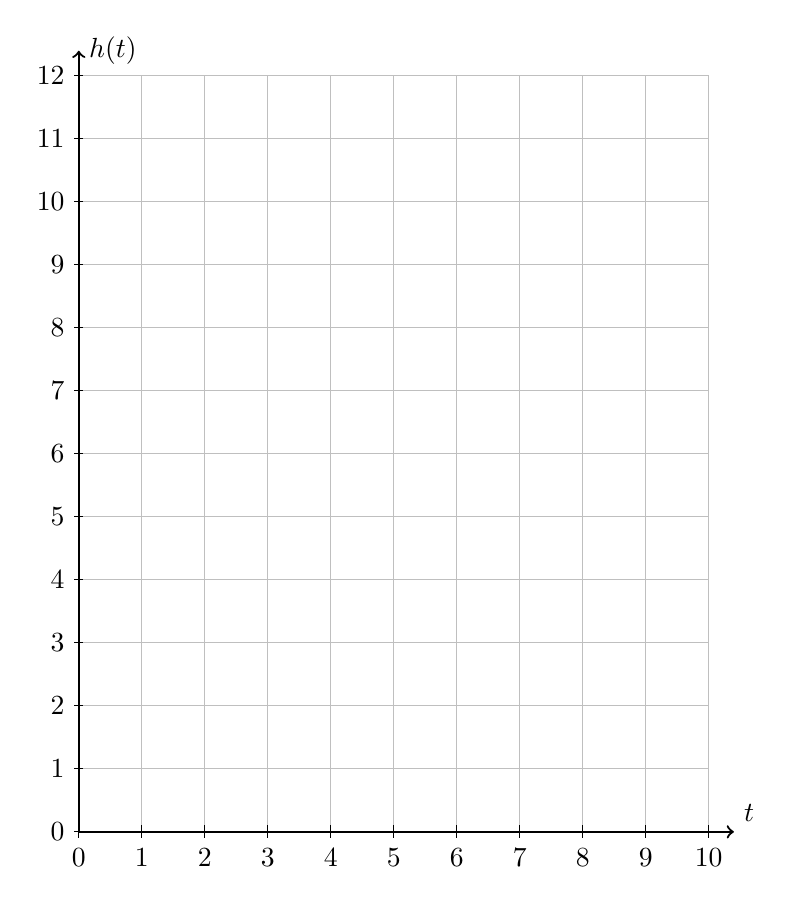
\begin{tikzpicture}[scale=0.8]
        \draw [thin, color=lightgray,, xstep=1.0cm,ystep=1.0cm] (0,0) grid (10,12);
        \foreach \x in {0,1,2,...,10}
        \draw (\x cm,3pt) -- (\x cm,-3pt) node[below] {$\x$};
        \foreach \y in {0,1,2,...,12}
        \draw[shift={(0,\y)},color=black] (2pt,0pt) -- (-2pt,0pt) node[left]  {$\y$};
        \draw [thick, ->] (0,0) -- (+10.4,0) node [above right] {$t$};
        \draw [thick, ->] (0,0) -- (0,12.4) node [right] {$h(t)$};
        %\draw [thick, <->,smooth,domain=-3.5:8.5] plot(\x,0.4*\x*\x-2*\x-8);
    \end{tikzpicture}
    \end{center}

\newpage
\item Given the arithmetic sequence $3,7,11,15,19, \dots$ \hfill [6]
    \begin{enumerate}[itemsep=1cm]
    \item Find the common difference $d$.
    \item Write down the next term, $u_6$.
    \item Find the twelfth term.\vspace{1cm}
    \item Find the sum of the first twelve terms.
    \end{enumerate} \vspace{2cm}

    \item The second term of an arithmetic sequence is 19 and the sixth term is 7. \hfill [6]
    \begin{enumerate}[itemsep=3cm]
    \item Find the common difference $d$.
    \item Find the first term, $u_{1}$.
    \item Find the sum of the first six terms.
    \end{enumerate} \vspace{2cm}

\item Given $f(x)=\frac{3}{5}x-3$.  \hfill [3]
\begin{enumerate}
    \item Find $f(10)$. \vspace{2cm}
    \item Find$f^{-1}(0)$.
\end{enumerate}

\newpage
Equations of a straight line: $f(x)=mx+c$, $ax+by+d=0$, $(y-y_1)=m(x-x_1)$\\[0.25cm]
Gradient: $\displaystyle m=\frac{y_2-y_1}{x_2-x_1}$ \vspace{1cm}

Arithmetic sequences\\[0.25cm]
Terms: $u_n=u_1 + d(n-1)$\\[0.25cm]
Sum: $\displaystyle S_n= \frac{n}{2}(u_1 + u_n)$\\[0.25cm]

Useful forms of equations for quadratics:\\[0.25cm] 
$f(x)=ax^2 + bx+c$, with $y$-intercept $c$, axis of symmetry $\displaystyle x=-\frac{b}{2a}$, zeros $\displaystyle x=\frac{-b \pm \sqrt{b^2-4ac}}{2a}$\\[0.25cm]
$g(x)=a(x-p)(x-q)$, with $x$-intercepts $p$, $q$ and axis of symmetry $\displaystyle x=\frac{p+q}{2}$\\[0.25cm] 
$h(x)=a(x-h)^2+k$, with vertex $(h,k)$


\end{enumerate}
\end{document}